\documentclass[11pt]{"article"}
\setlength{\parindent}{0pt}
\linespread{1.5}
\usepackage[margin=1in]{geometry}
\usepackage{graphicx}
\graphicspath{ {../Figures/} }
\usepackage{titlesec}
\newcommand{\sectionbreak}{\clearpage}
\usepackage{sidecap}
\usepackage[singlelinecheck=false, labelfont=bf]{caption}
\usepackage{verbatim}
\usepackage{setspace}
\newcommand{\mycaption}[2]{\caption[#1]{\textbf{#1.} #2}}
\usepackage{chngcntr}
\counterwithin{figure}{section}


\begin{document}

\begin{titlepage}
\centering
{\huge Title\\}
\end{titlepage}


\pagebreak

\begin{Large}
\textbf{Abstract}\\
\end{Large}


\pagebreak

\begin{Large}
\textbf{Impact statement}\\
\end{Large}


\pagebreak

\begin{Large}
\textbf{Acknowledgements}\\
\end{Large}


\tableofcontents
\listoffigures


%%%%%%%%%%%%%%%%%%%%%%%%%%%%%%%%%%%%%%%%%%%%%%%%%%%%%%%%%%
\clearpage
\section{Introduction}

\subsection{Spatial patterning in biological systems}

\clearpage
\subsection{Cell polarity}

\clearpage
\subsection{Maintenance of cell polarity by bistable reaction-diffusion systems}
\subsubsection{Bistable reaction kinetics}
\subsubsection{Single species polarity models}
\subsubsection{The mutual antagonism model}

\clearpage
\subsection{A molecular basis for ultrasensitivity}
\subsubsection{Ultrasensitivity in protein phosphorylation reactions}
\subsubsection{Ultrasensitivity through cooperative membrane binding}

\clearpage
\subsection{PAR polarity in C elegans zygotes}
\subsubsection{Mechanisms of PAR cortical association}
\subsubsection{Maintenance of polarity by mutual antagonism}
\subsubsection{Establishment of polarity}
\subsubsection{Downstream of the PAR proteins}
\subsubsection{Resistance and substrate competition}
\subsubsection{Discussion}

\clearpage
\subsection{PAR-2: roles and mechanisms of action}
\subsubsection{Main functional roles of PAR-2}
\subsubsection{Evidence and proposed roles for oligomerisation}
\subsubsection{Roles for the RING domain}

\clearpage
\subsection{RING domains across the proteome}
\subsubsection{RING proteins in the ubiquitination pathway}
\subsubsection{RINGs as dimerisation domains}
\subsubsection{Discussion}

%%%%%%%%%%%%%%%%%%%%%%%%%%%%%%%%%%%%%%%%%%%%%%%%%%%%%%%%%%
\clearpage
\section{A pipeline for quantification of membrane and cytoplasmic protein concentrations}

Text

\subsection{Autofluorescence correction}
\subsubsection{Autofluorescence in C elegans}
\subsubsection{Spectral imaging for autofluorescence correction}
\subsubsection{SAIBR: a tool for spatial autofluorescence correction}

\begin{figure}[!h]
\includegraphics[scale=1]{saibr_n2_correlation}
\setlength{\abovecaptionskip}{20pt}
\centering
\mycaption{Title}{Caption}
\end{figure}


\begin{figure}[!h]
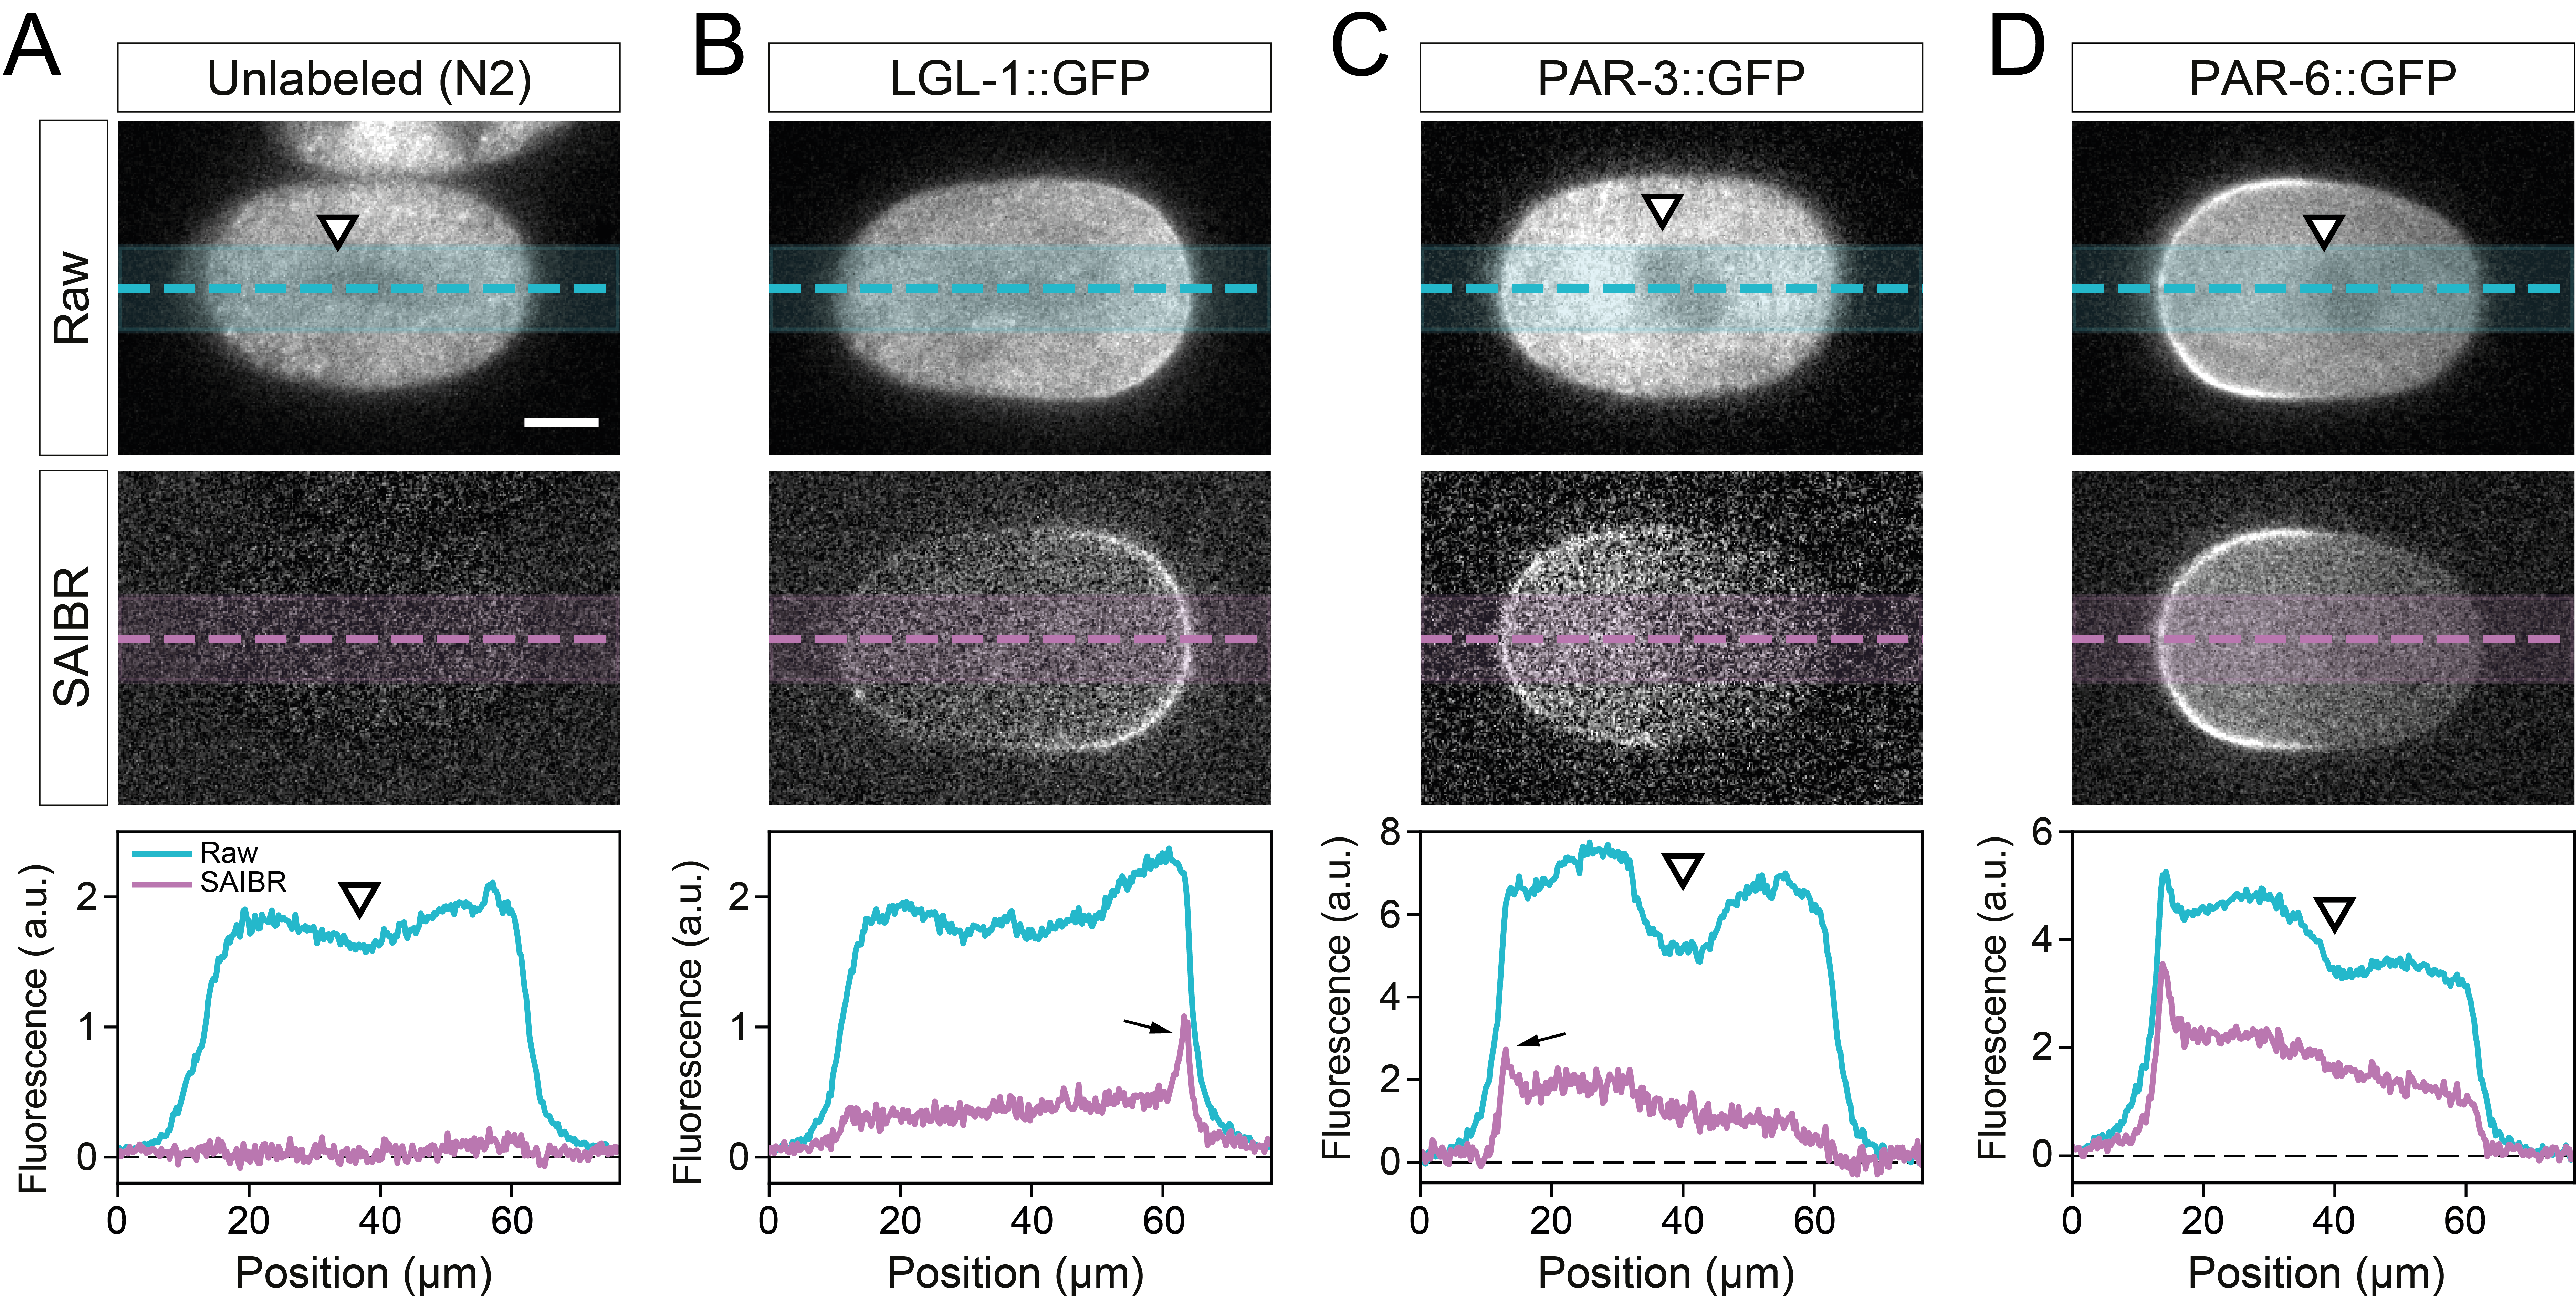
\includegraphics[scale=1]{saibr_spatial_correction}
\setlength{\abovecaptionskip}{20pt}
\centering
\mycaption{Title}{Caption}
\end{figure}

\begin{figure}[!h]
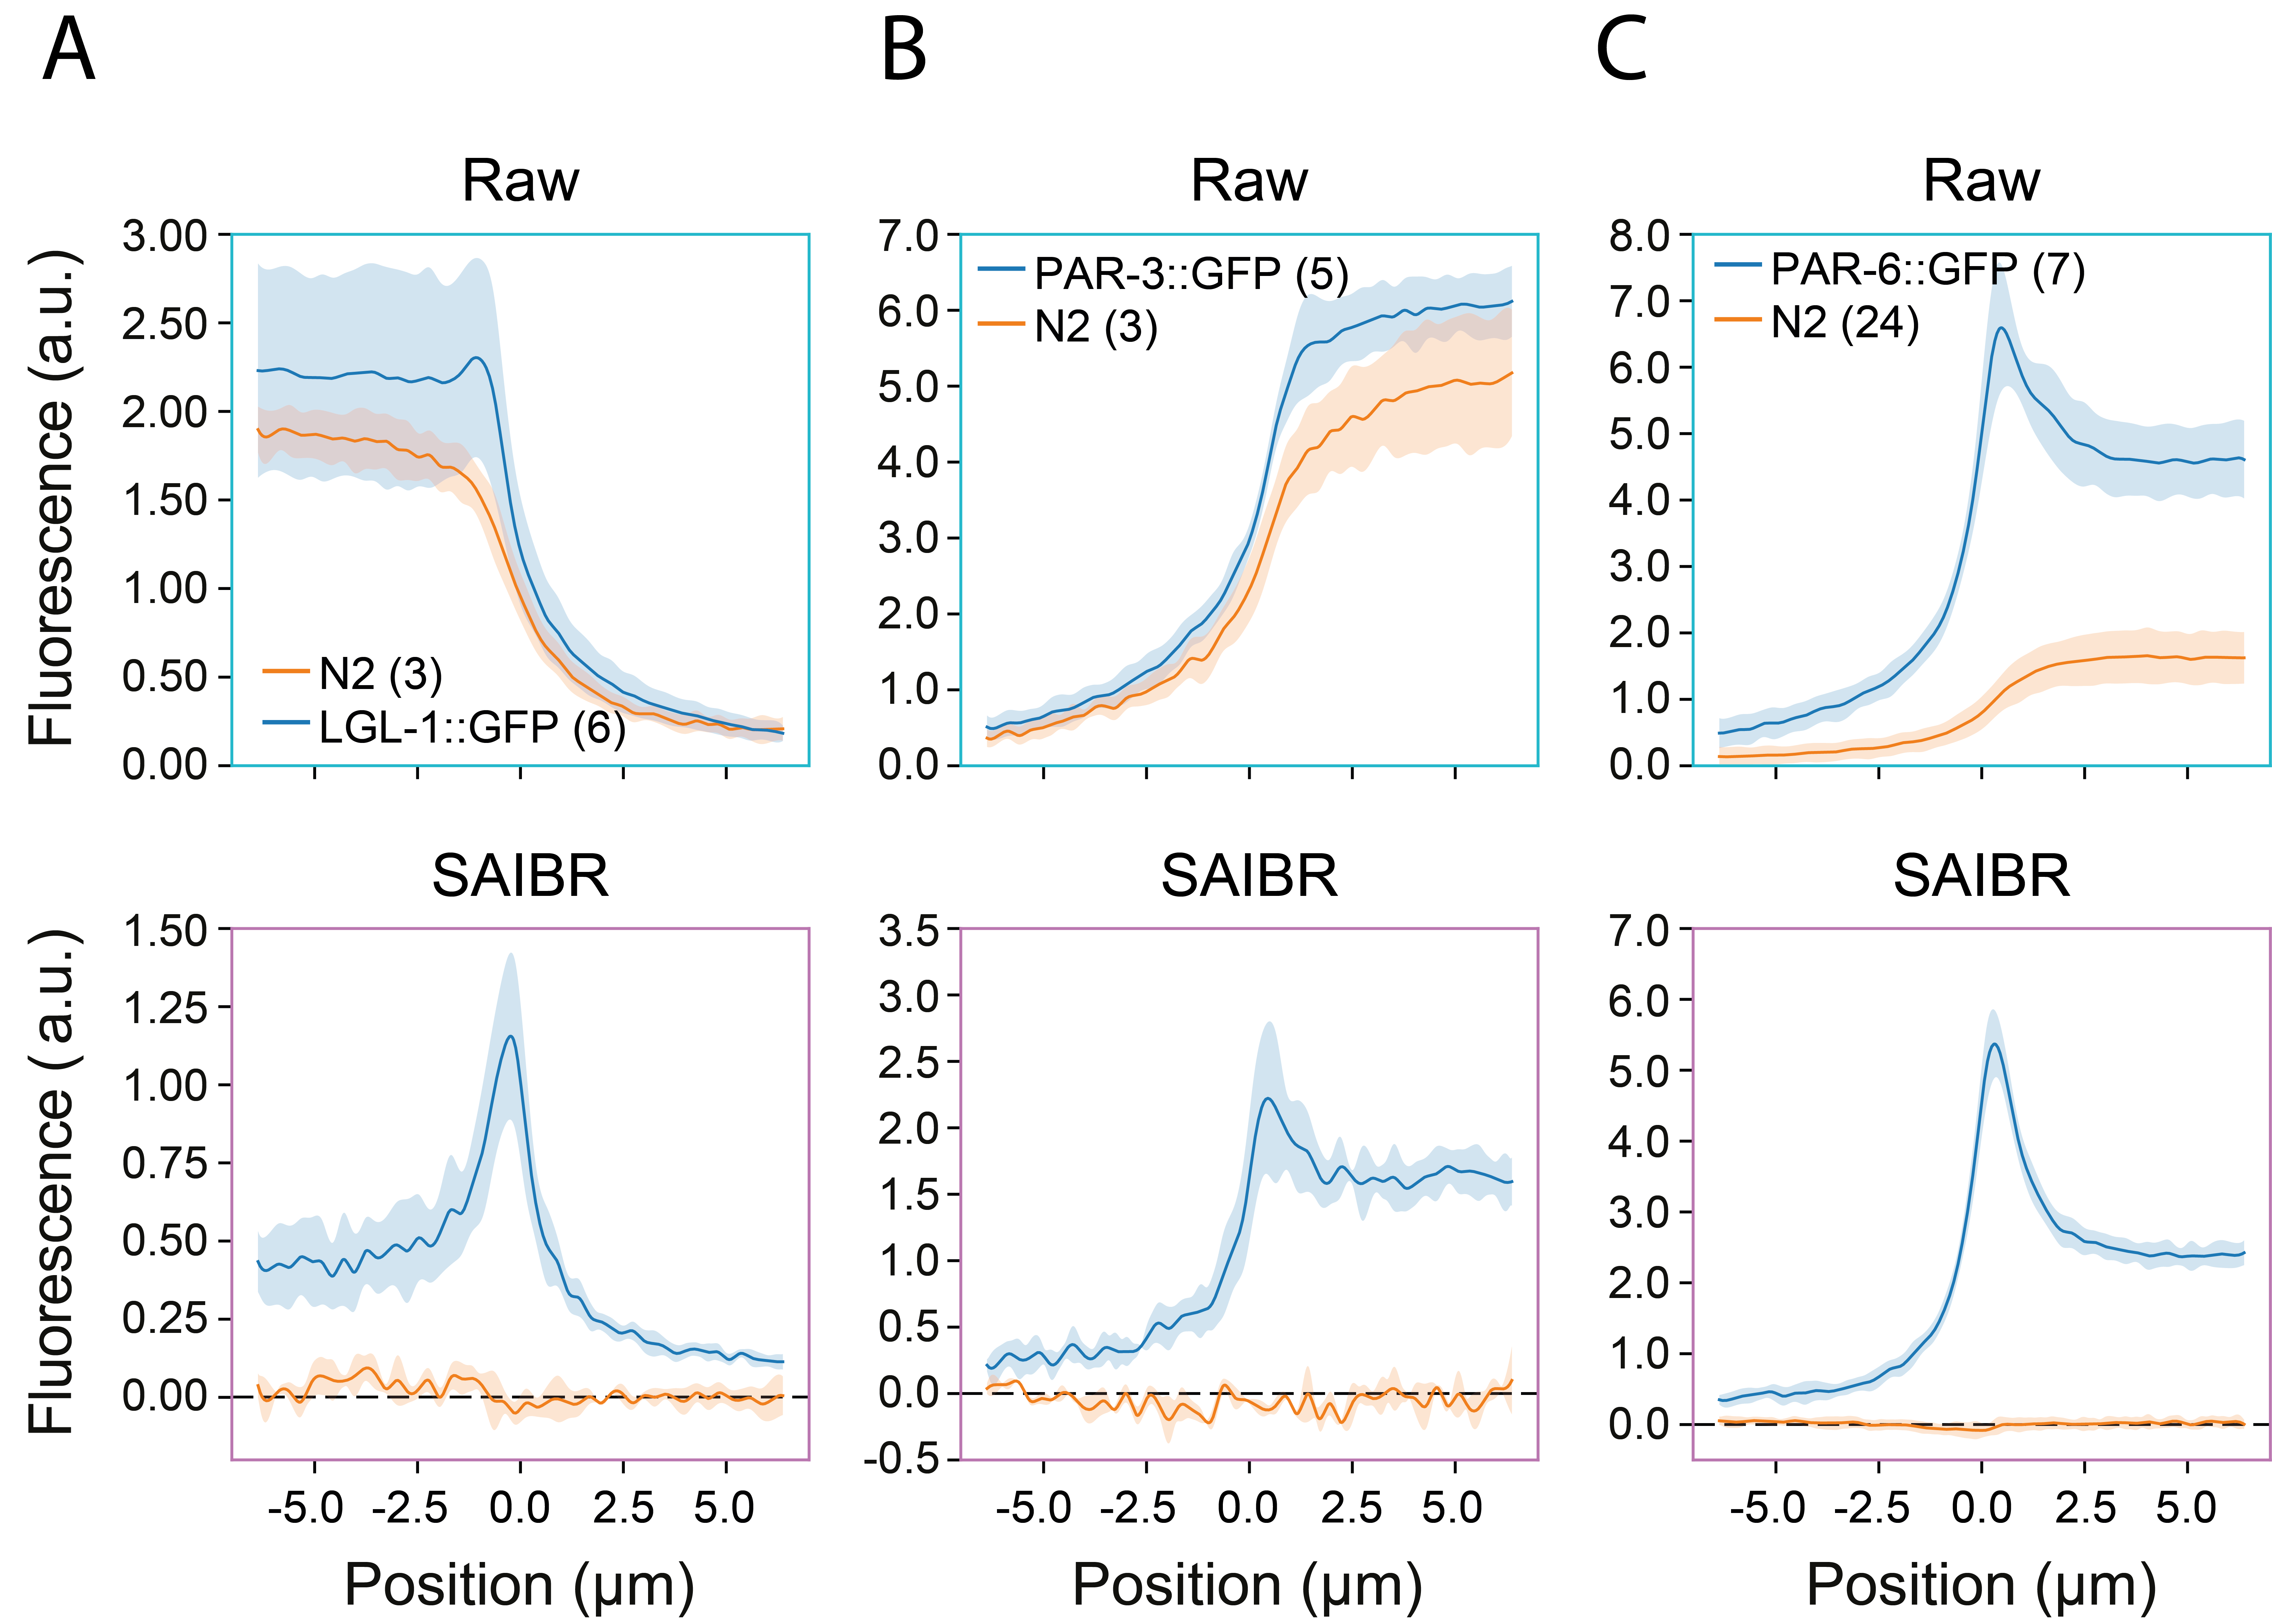
\includegraphics[scale=1]{saibr_membrane_profiles}
\setlength{\abovecaptionskip}{20pt}
\centering
\mycaption{Title}{Caption}
\end{figure}

\clearpage
\subsubsection{Autofluorescence correction in two-colour samples}

\begin{figure}[!h]
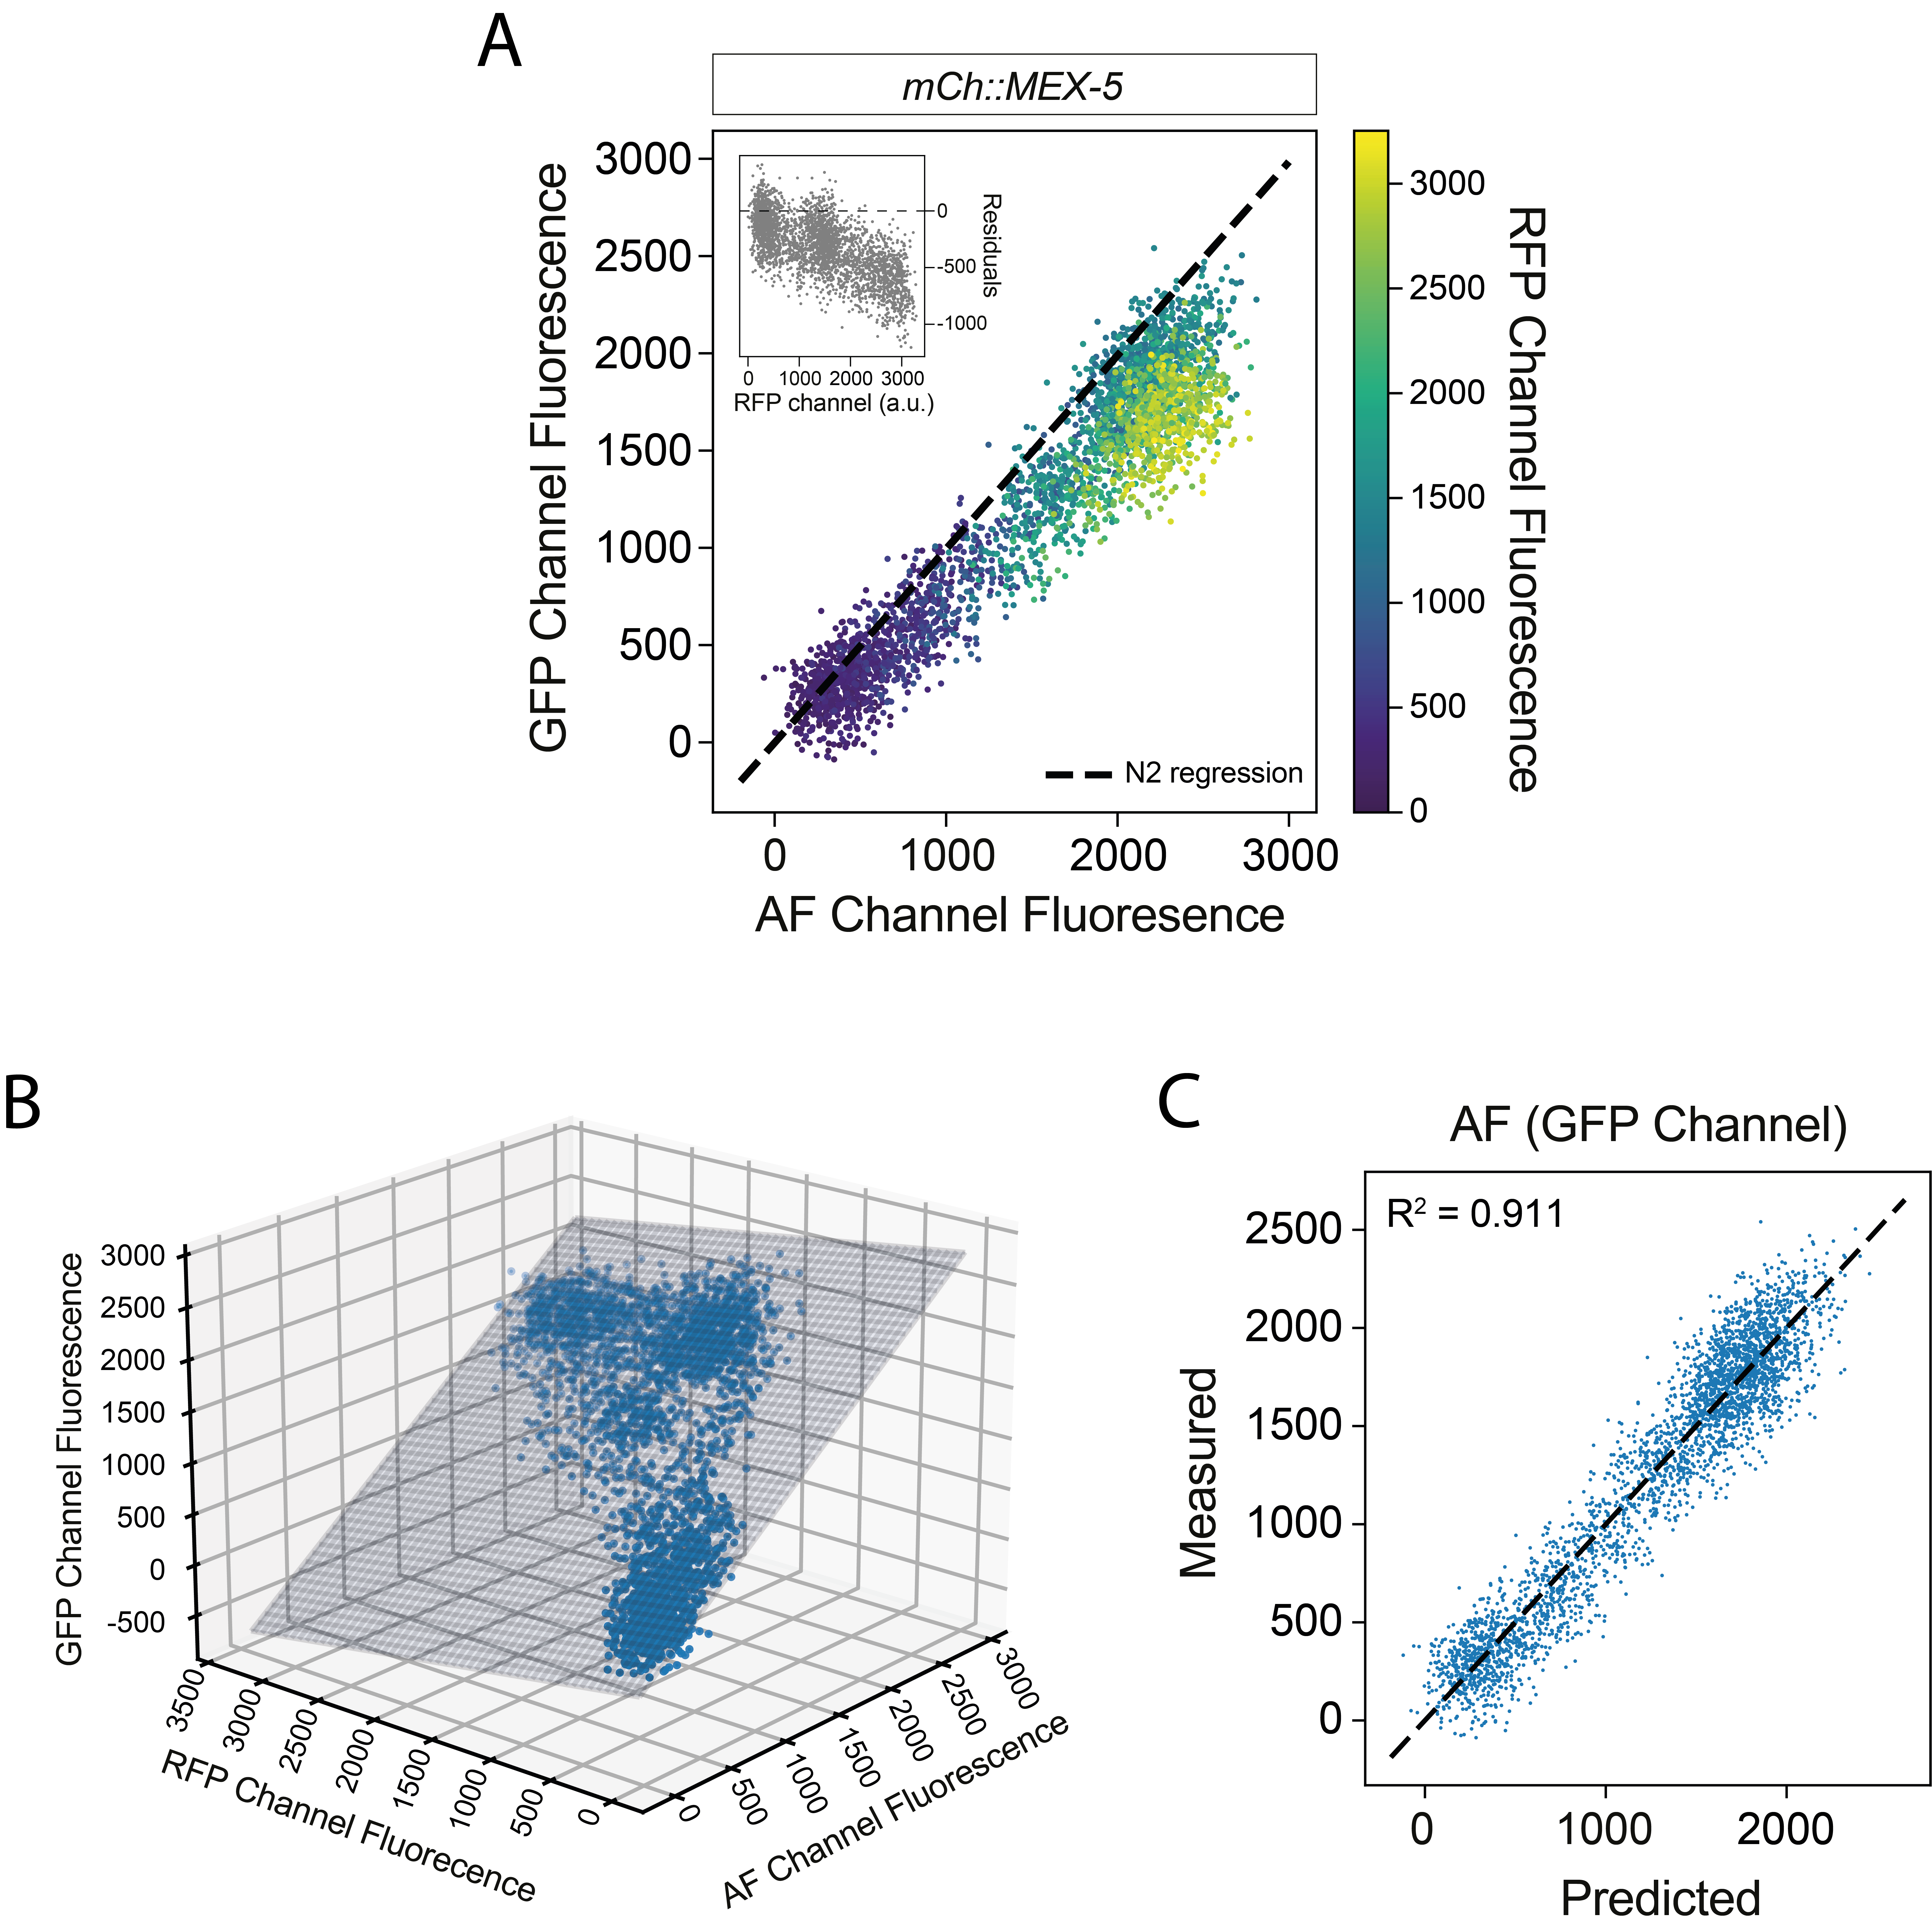
\includegraphics[scale=1]{saibr_3channel_correlation}
\setlength{\abovecaptionskip}{20pt}
\centering
\mycaption{Title}{Caption}
\end{figure}

\begin{figure}[!h]
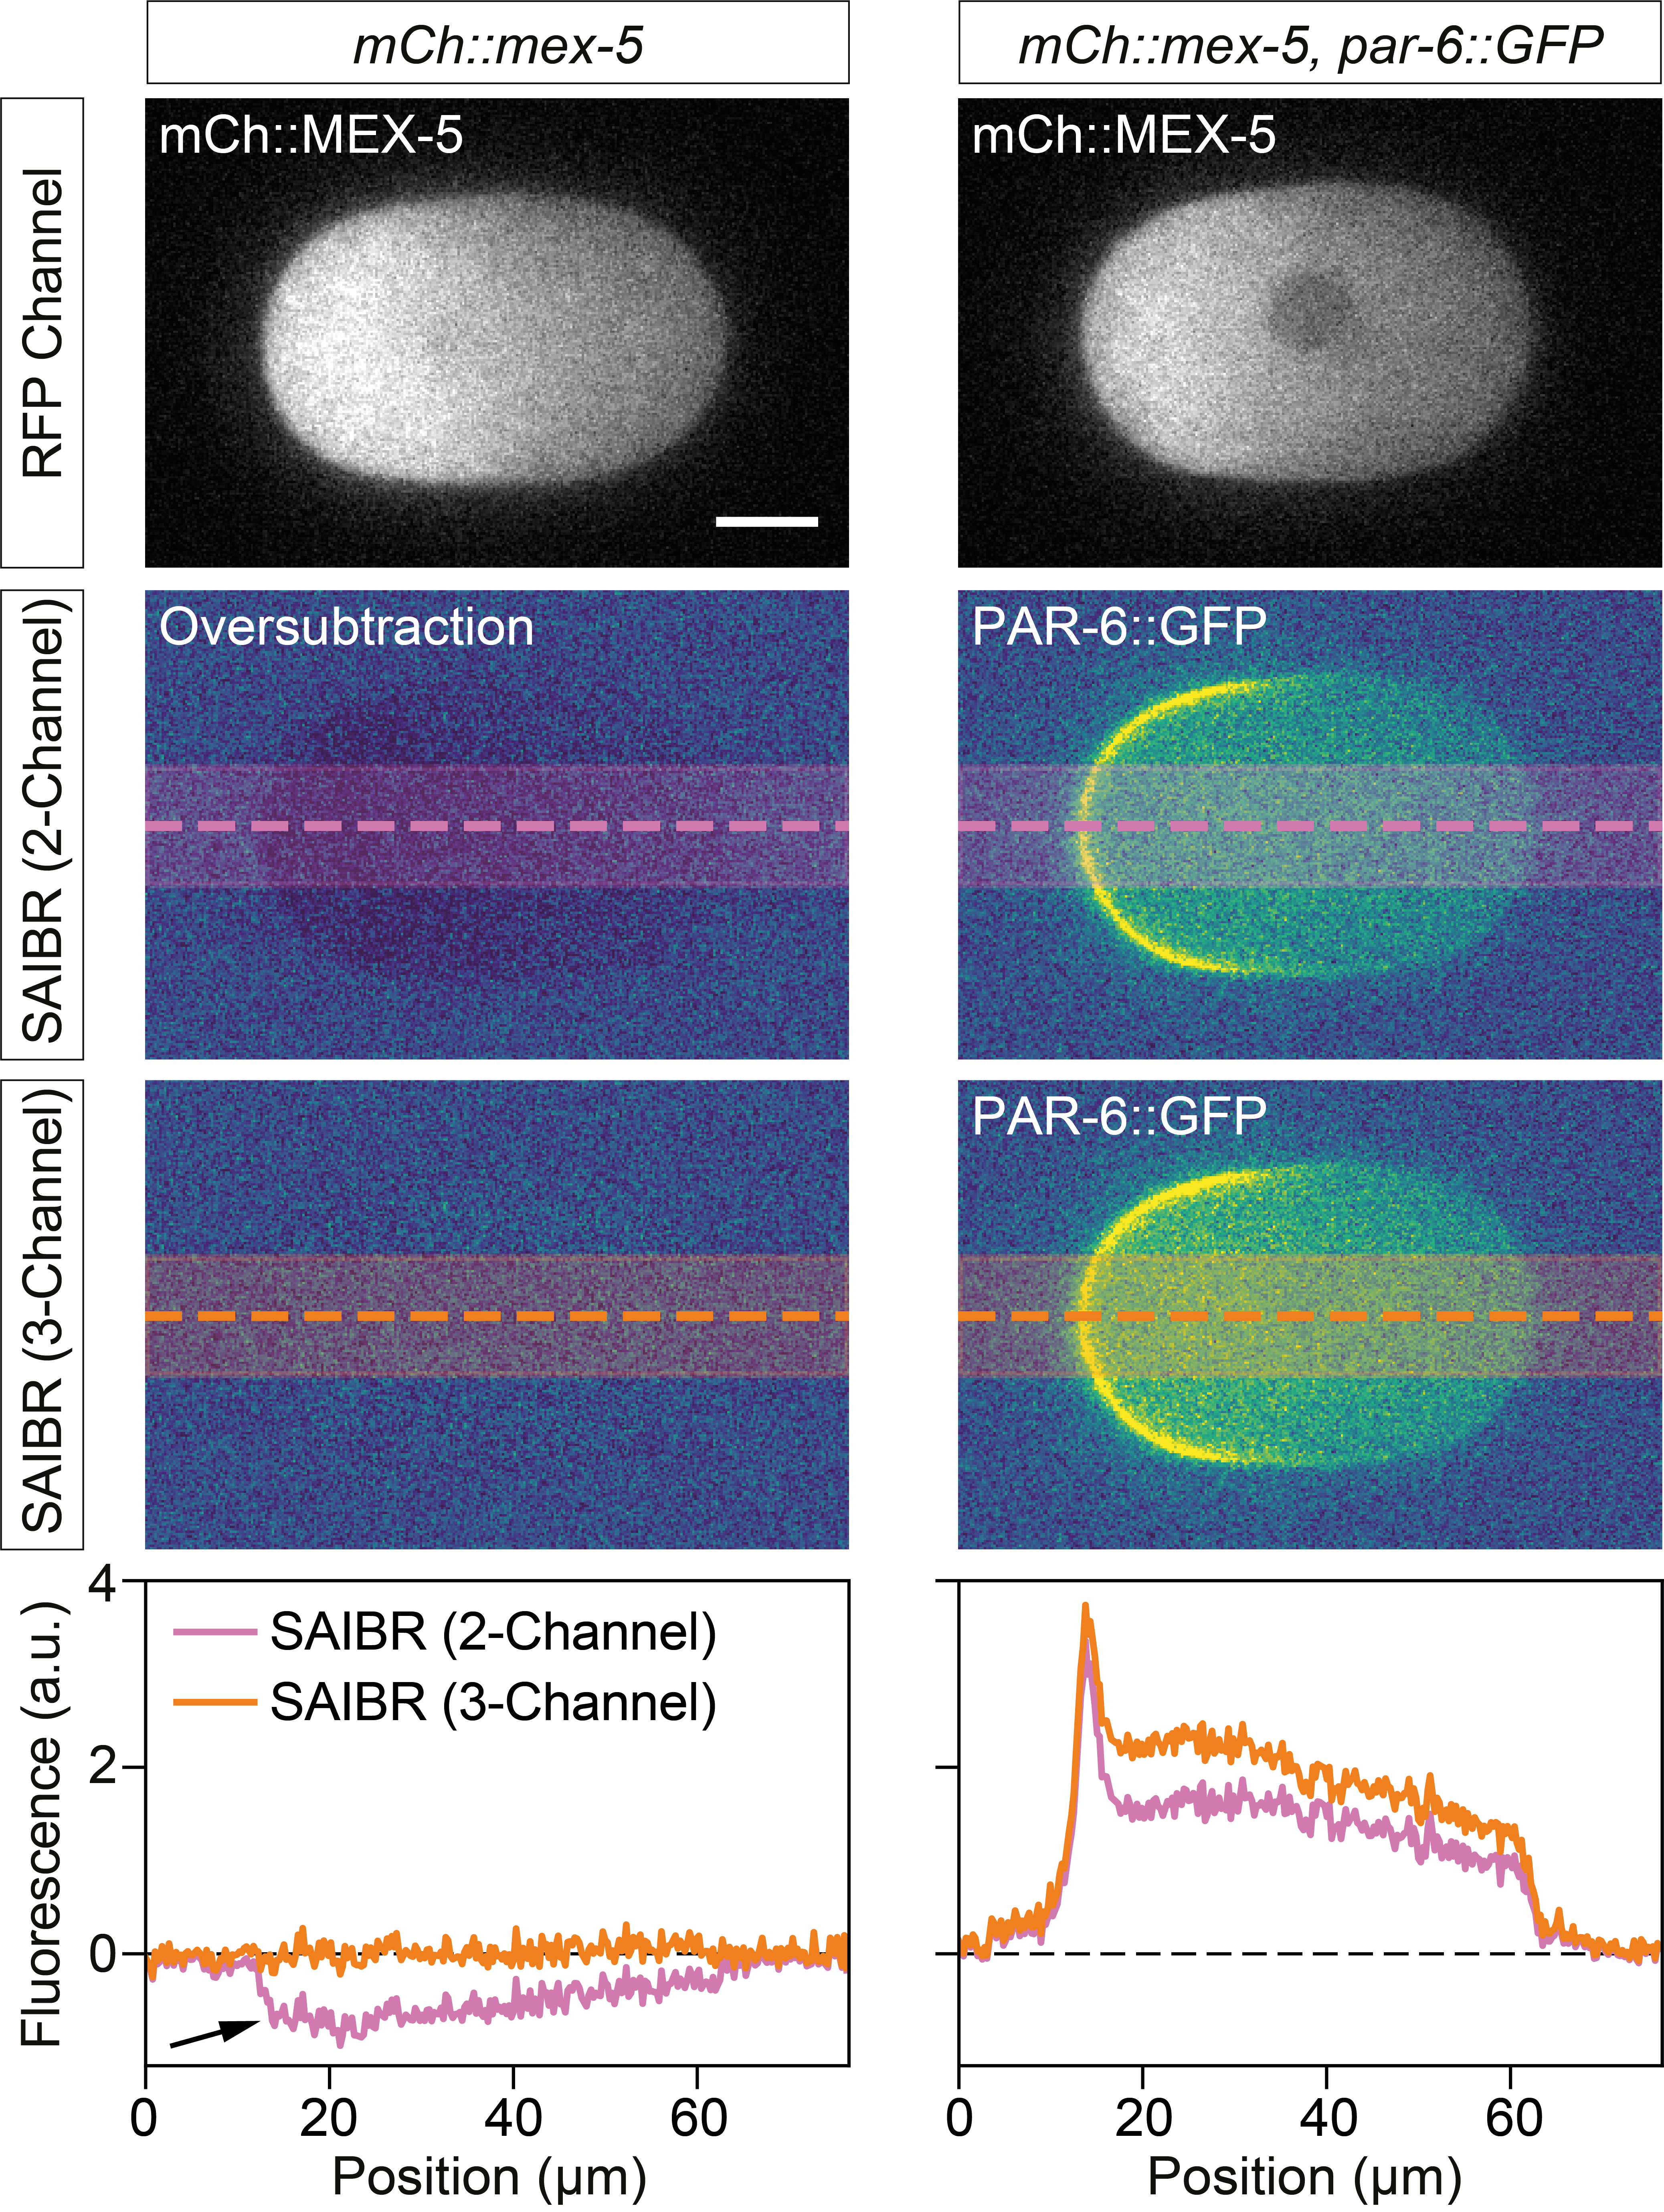
\includegraphics[scale=0.9]{saibr_3channel_correction}
\setlength{\abovecaptionskip}{20pt}
\centering
\mycaption{Title}{Caption}
\end{figure}

\clearpage
\subsubsection{Discussion}

\clearpage
\subsection{Extraction of membrane and cytoplasmic signal components}


\begin{figure}[!h]
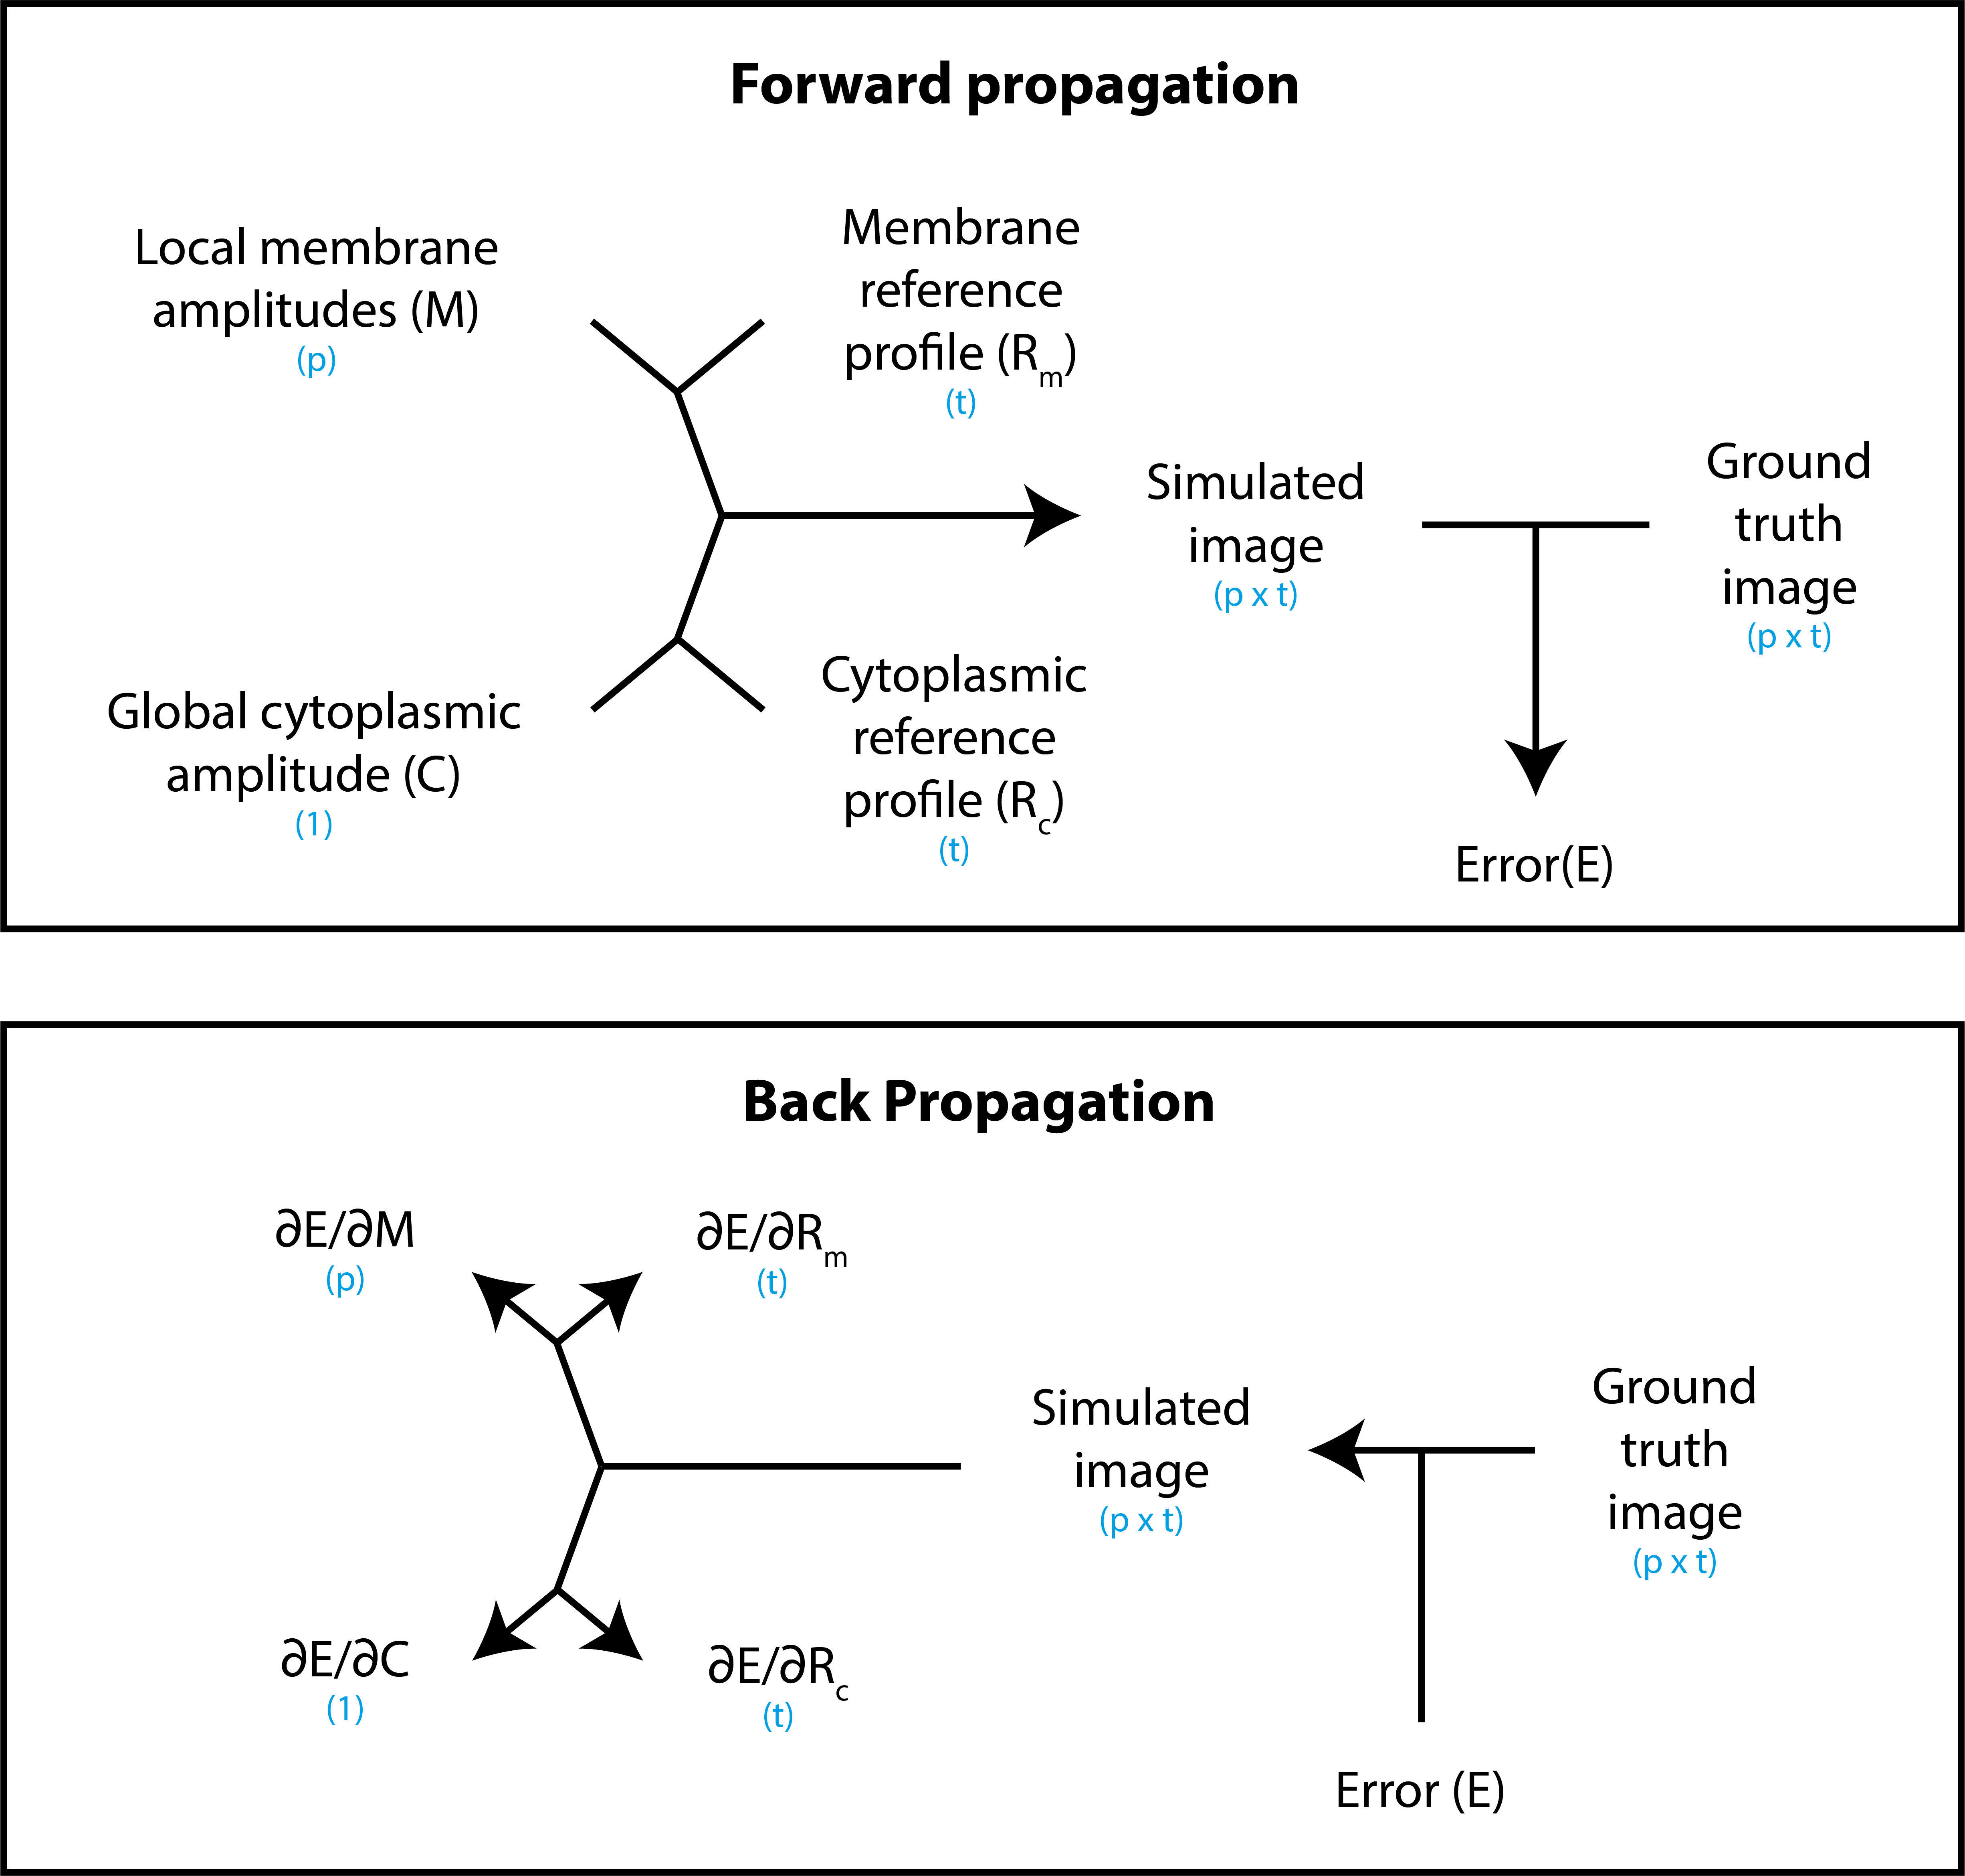
\includegraphics[scale=1]{memquant_forward_and_back_propagation}
\setlength{\abovecaptionskip}{20pt}
\centering
\mycaption{Title}{Caption}
\end{figure}

\begin{figure}[!h]
\includegraphics[scale=1]{memquant_membg_training}
\setlength{\abovecaptionskip}{20pt}
\centering
\mycaption{Title}{Caption}
\end{figure}

\clearpage
\subsubsection{Segmentation}


\clearpage
\subsubsection{Benchmarking the method}

\begin{figure}[!h]
\includegraphics[scale=1]{memquant_benchmarking_ph_rundown}
\setlength{\abovecaptionskip}{20pt}
\centering
\mycaption{Title}{Caption}
\end{figure}

\begin{figure}[!h]
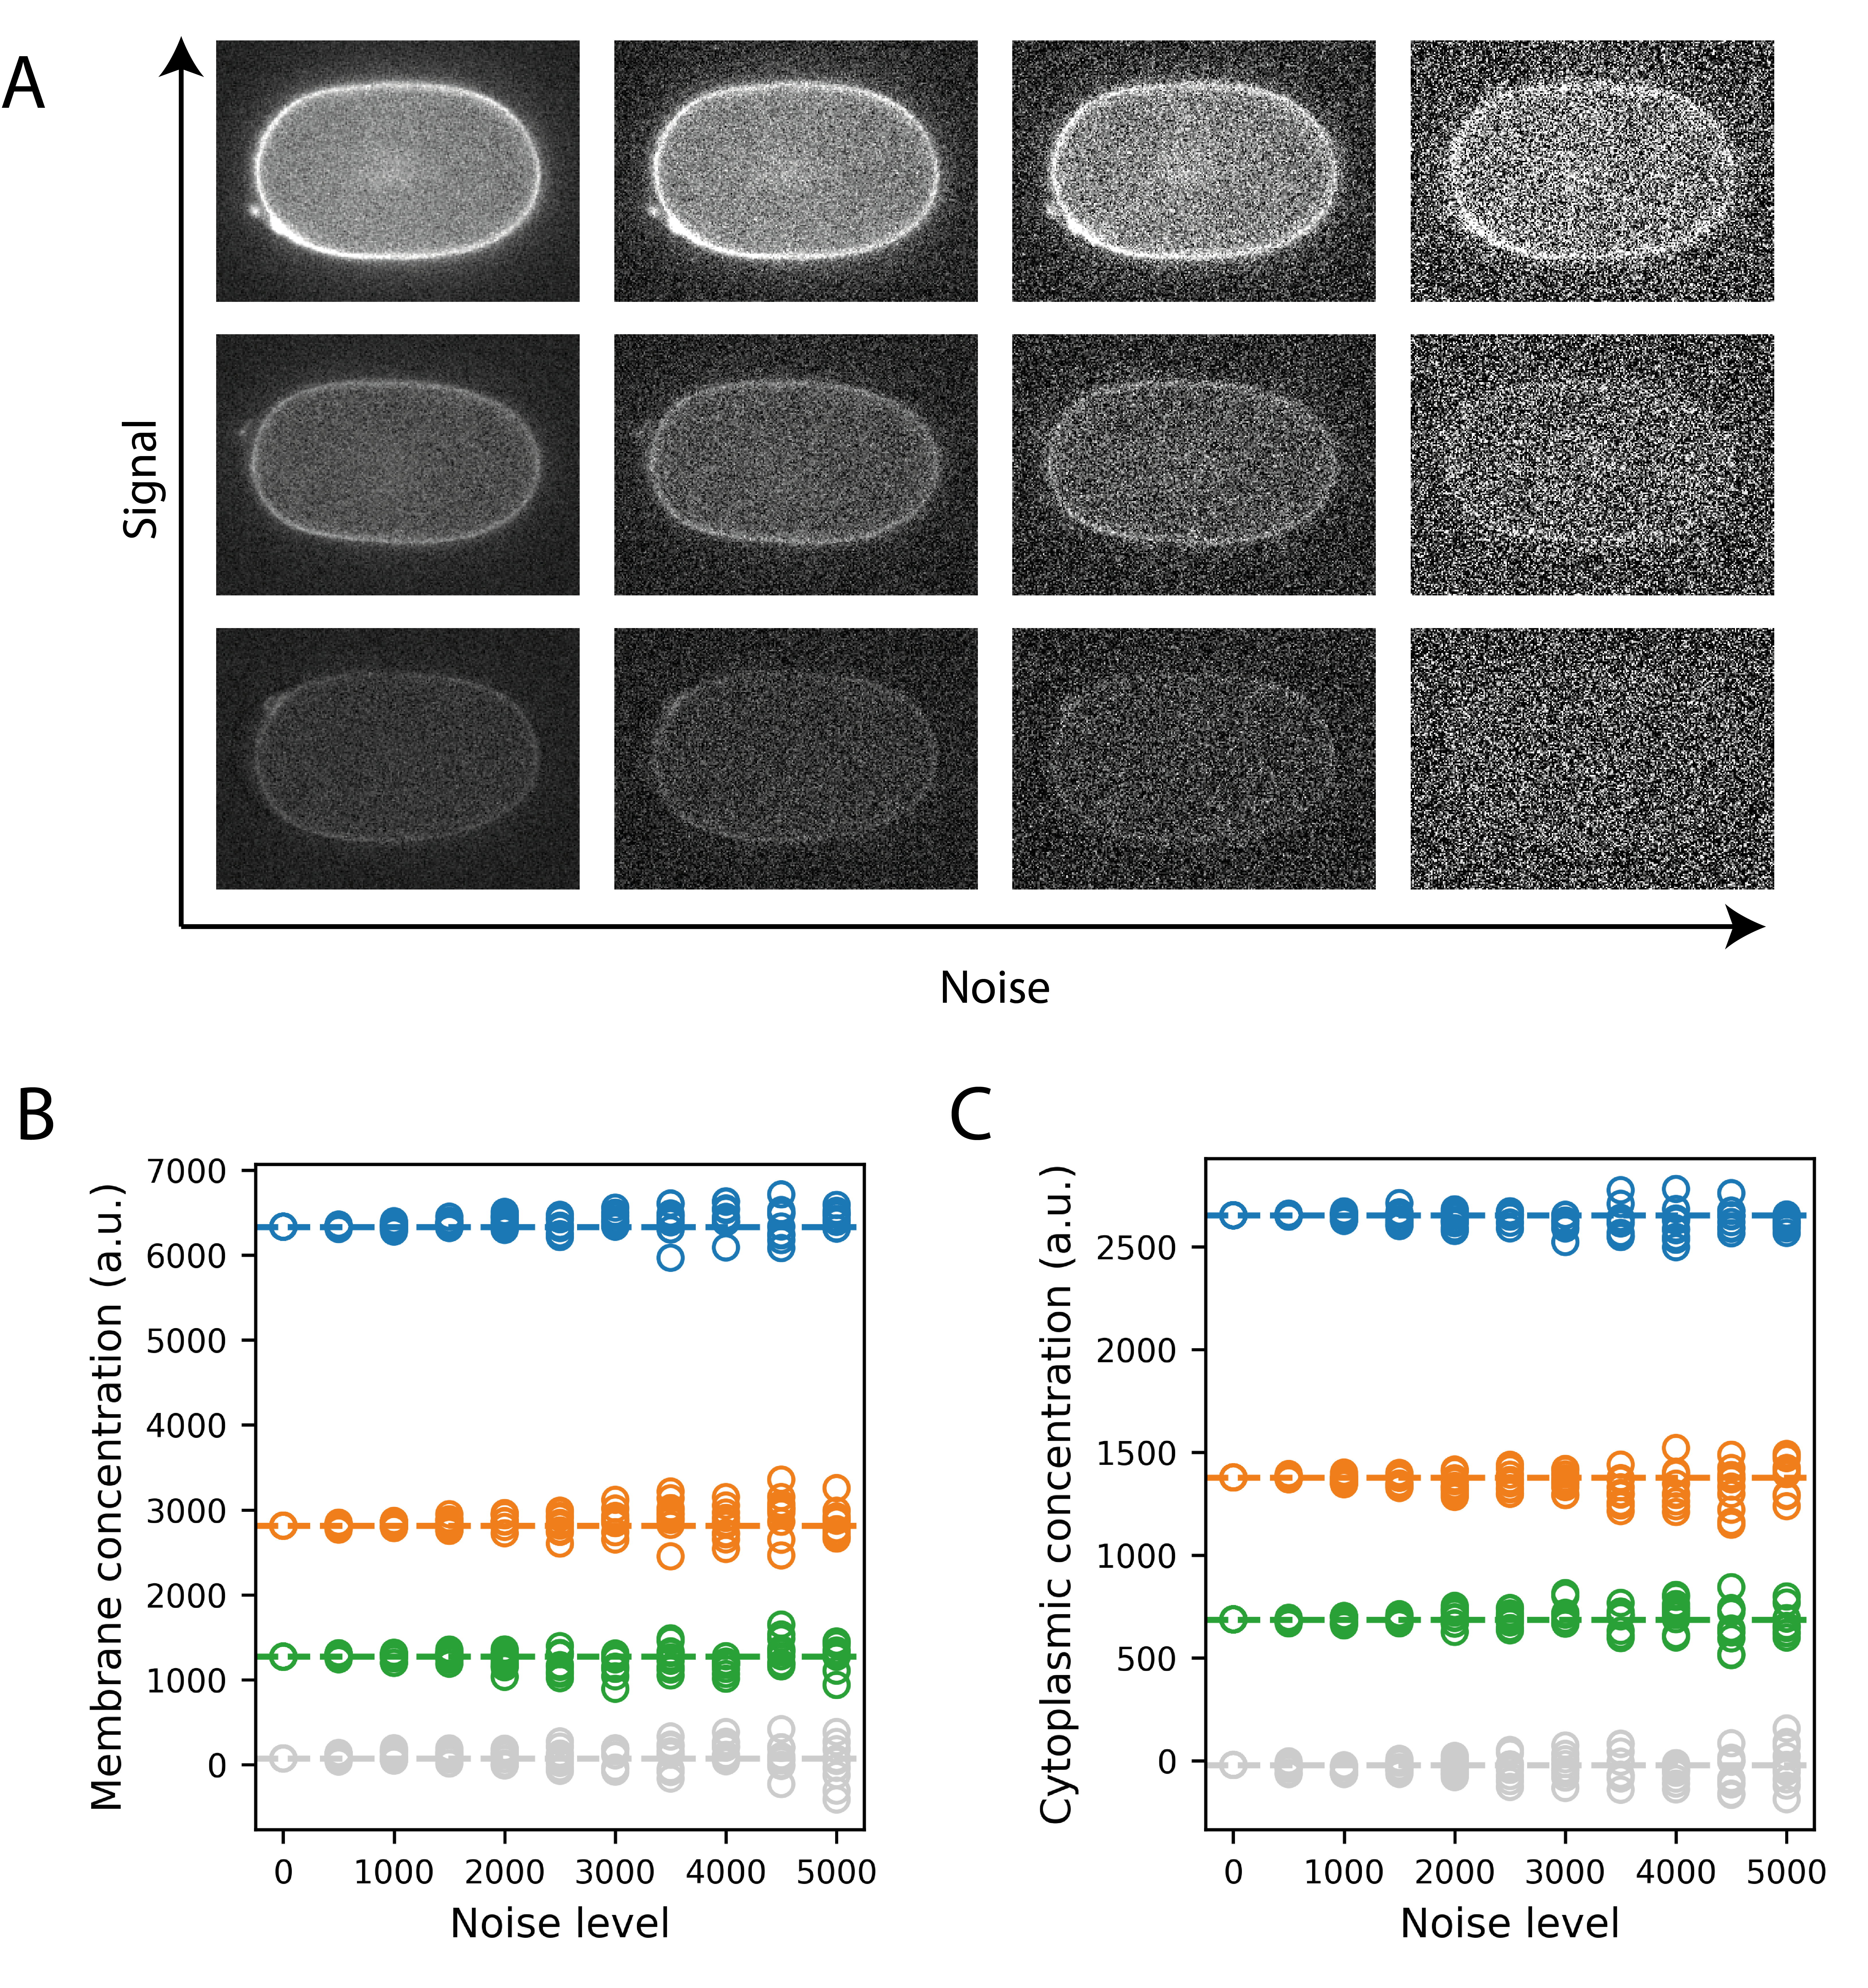
\includegraphics[scale=1]{memquant_benchmarking_noise}
\setlength{\abovecaptionskip}{20pt}
\centering
\mycaption{Title}{Caption}
\end{figure}


\clearpage
\subsubsection{Calibration of concentration units}

\begin{figure}[!h]
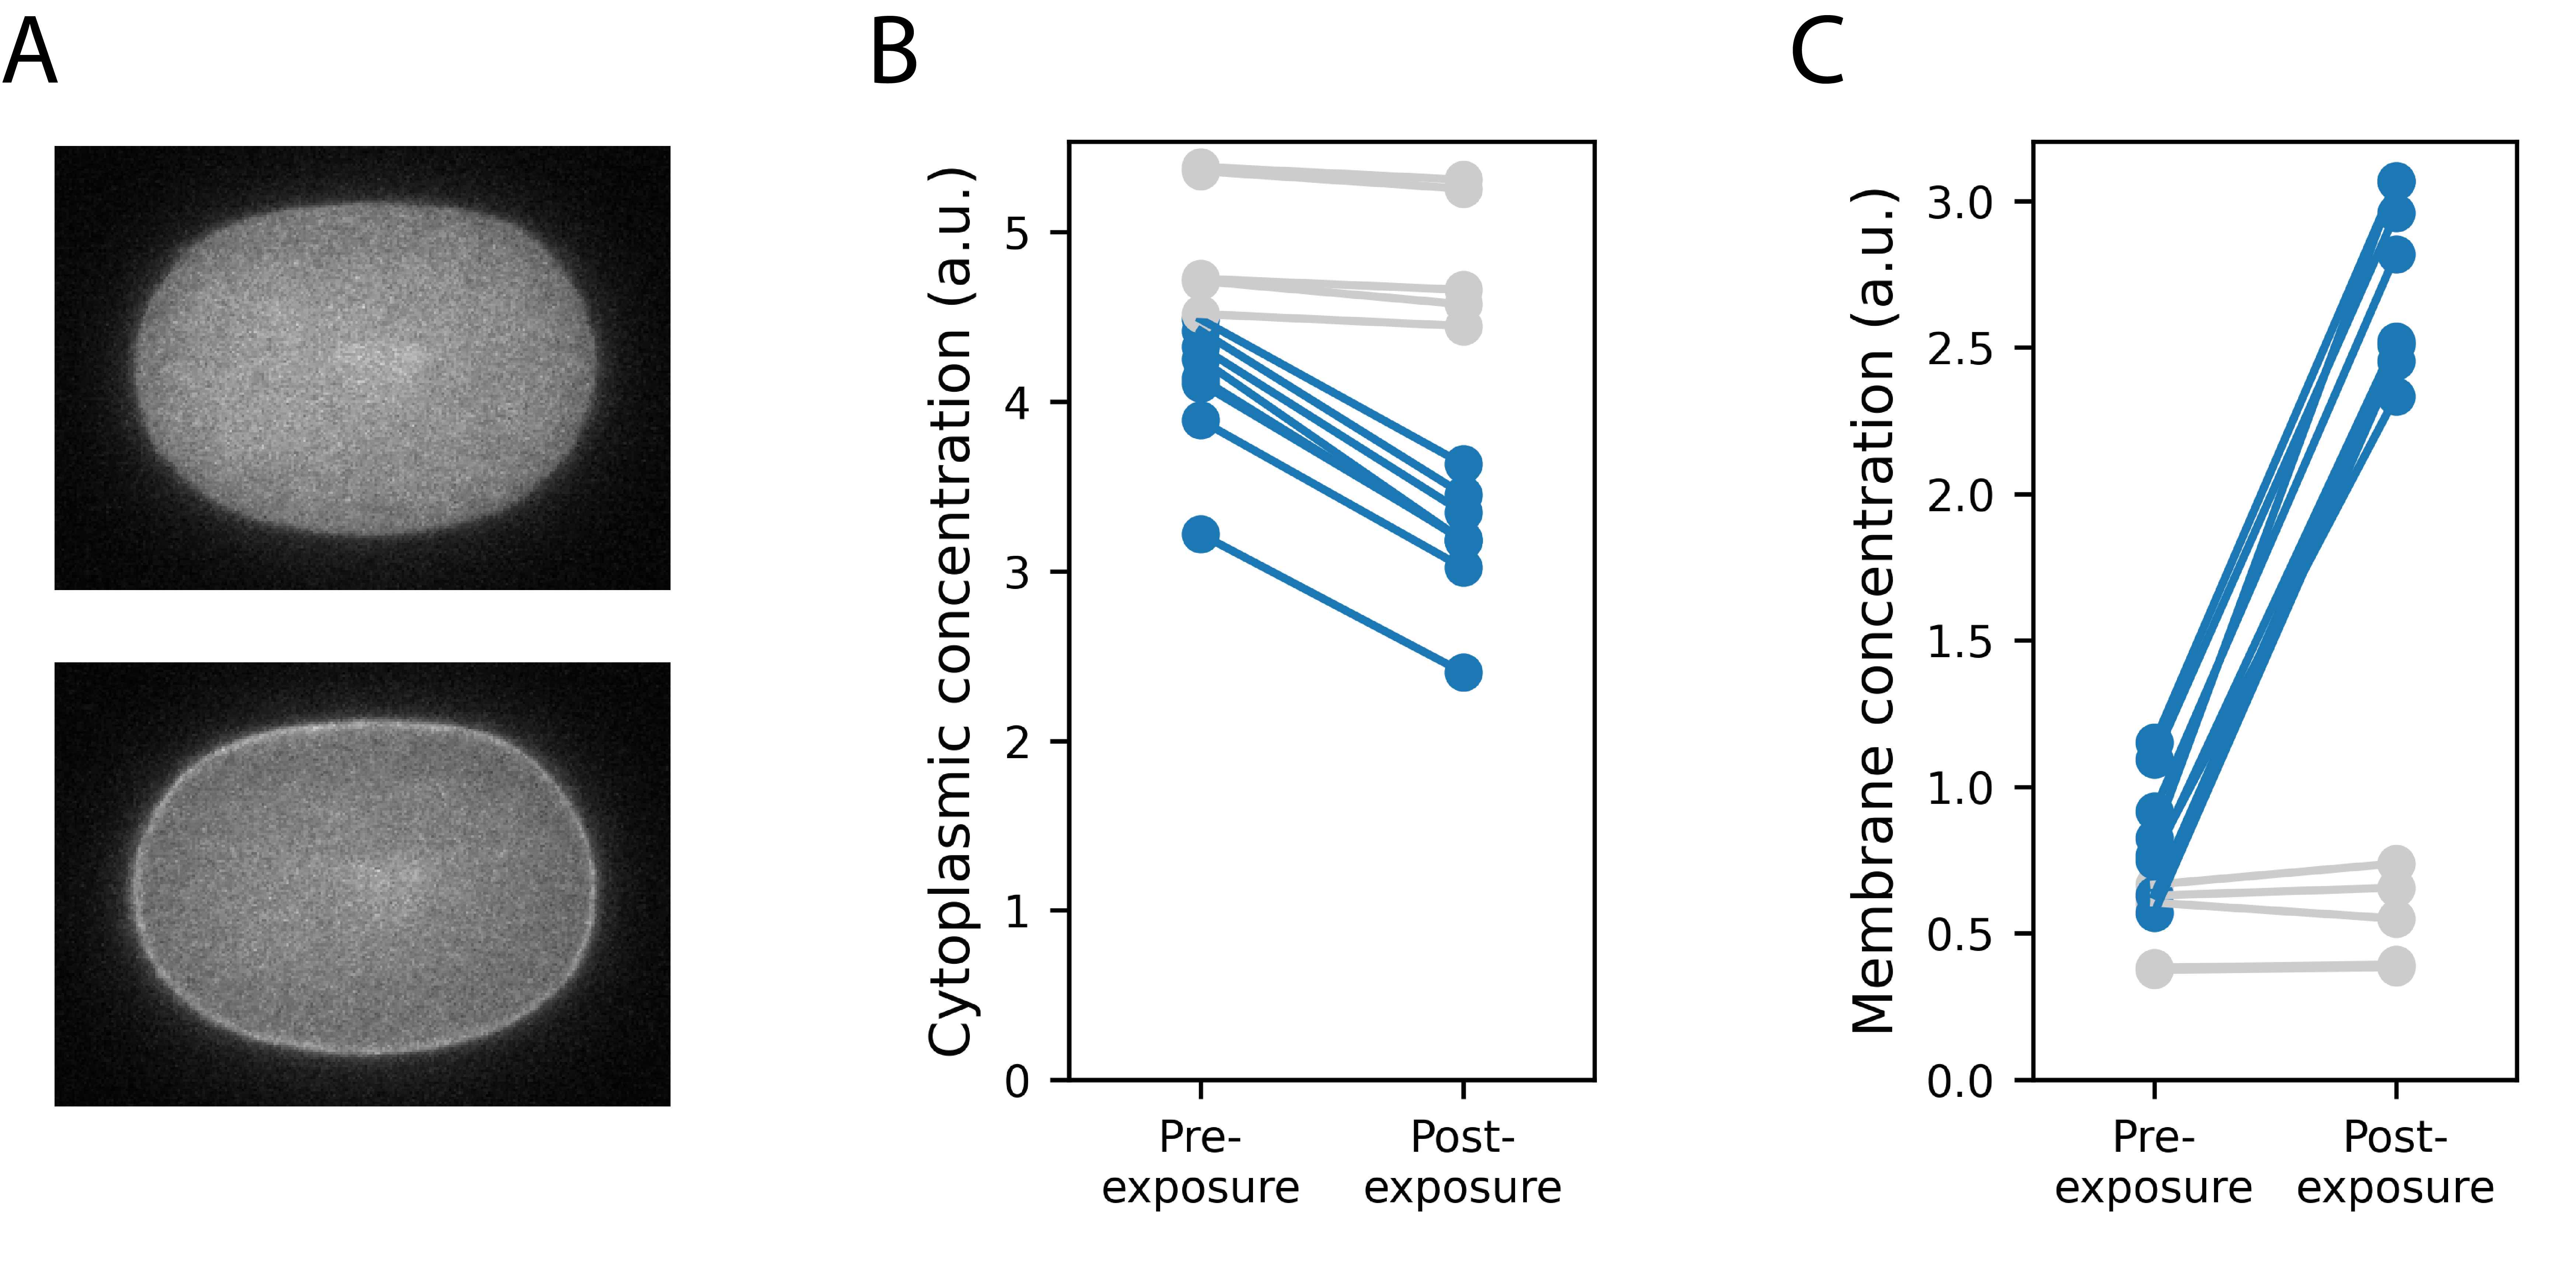
\includegraphics[scale=1]{memquant_optogenetics}
\setlength{\abovecaptionskip}{20pt}
\centering
\mycaption{Title}{Caption}
\end{figure}

\clearpage
\subsubsection{Discussion}

%%%%%%%%%%%%%%%%%%%%%%%%%%%%%%%%%%%%%%%%%%%%%%%%%%%%%%%%%%
\clearpage
\section{Identifying core patterning behaviours of PAR-2}

Text

\subsection{PAR-2 polarity in systems with uniform aPAR}

\subsection{Polarity phenotypes in PAR-2 mutants}

\subsection{Quantitative characterisation of PAR-2 mutants}

\subsection{Discussion}

%%%%%%%%%%%%%%%%%%%%%%%%%%%%%%%%%%%%%%%%%%%%%%%%%%%%%%%%%%
\clearpage
\section{Determining the mechanisms of PAR-2 RING domain action}

Text

\subsection{Exploring a role for ubiquitination}
\subsubsection{PAR-2 purification and in vitro ubiquitination assays}
\subsubsection{Sequence analysis and targeted mutation of putative linchpin site}

\subsection{Exploring a role for dimerisation}
\subsubsection{Structure prediction}
\subsubsection{Characterising dimerisation in vitro}
\subsubsection{Characterising dimerisarion in vivo}
\subsubsection{Targeted mutation to dimerisation interface regions}

\subsection{Discussion}


%%%%%%%%%%%%%%%%%%%%%%%%%%%%%%%%%%%%%%%%%%%%%%%%%%%%%%%%%%
\clearpage
\section{A thermodynamic model of PAR-2 dimerisation}

Text

\subsection{Model description}

\subsection{Dimerisation-driven positive feedback}

\subsection{Quantitative analysis of PAR-2 membrane binding kinetics}

\subsection{Discussion}

%%%%%%%%%%%%%%%%%%%%%%%%%%%%%%%%%%%%%%%%%%%%%%%%%%%%%%%%%%
\clearpage
\section{Direct experimental manipulation of dimerisation}

Text

%%%%%%%%%%%%%%%%%%%%%%%%%%%%%%%%%%%%%%%%%%%%%%%%%%%%%%%%%%
\clearpage
\section{Modelling dimerisation-driven positive feedback in the PAR network}

Text

%%%%%%%%%%%%%%%%%%%%%%%%%%%%%%%%%%%%%%%%%%%%%%%%%%%%%%%%%%
\clearpage
\section{Discussion}

Text

%%%%%%%%%%%%%%%%%%%%%%%%%%%%%%%%%%%%%%%%%%%%%%%%%%%%%%%%%%
\clearpage
\section{Materials and methods}

Text

\subsection{Worm maintenance}
\subsection{Generating transgenic lines by CRISPR}
\subsection{Microscopy}
\subsection{Full-length PAR-2 purification}
\subsection{Ubiquitination assays}
\subsection{PAR-2 RING domain fragment purification}
\subsection{SEC-MALS}
\subsection{Image analysis}
\subsection{Modelling methods}

%%%%%%%%%%%%%%%%%%%%%%%%%%%%%%%%%%%%%%%%%%%%%%%%%%%%%%%%%%
\clearpage
\section{Bibliography}

\end{document}
